\section{Datensatz und Use Cases}\label{sec:use_case}

Für die nachfolgenden Experimente werden zwei unterschiedliche Datenbestände genutzt: der CIFAR-10 Datenbestand \cite{cifar10} und der CelebA Datenbestand \cite{celeba}.
Bei dem CIFAR-10 Datenbestand handelt es sich um 60.000 Bilder, welche jeweils eine Auflösung von 32$\times$32 Pixeln, sowie je 3 Farbkanäle, haben.
Jedes Bild zeigt ein Objekt, welches genau einer von 10 Klassen zugeordnet werden kann. 
Bei diesen Klassen handelt es sich um Tierarten (beispielsweise \dq \textit{Hund}\dq oder \dq \textit{Katze}\dq) oder um Fahrzeugtypen (beispielsweise \dq \textit{Auto}\dq\ oder \dq \textit{Flugzeug}\dq).
Der Datenbestand ist bereits in \dq \textit{Training}\dq\ und \dq \textit{Test}\dq\ eingeteilt, wobei jede der 10 Klassen in beiden Datenmengen jeweils genau 10 \% einnimmt.
Der Use Case ist es nun, die Bilder der richtigen Klasse zuzuordnen.
Dafür wird ein Modell genutzt, welches eine ResNet-Architektur mit 10 Schichten nutzt \cite{resnet}.
Dabei handelt es sich um ein neuronales Netz, welches großteils aus Faltungsschichten, sowie einigen Pooling-Schichten besteht.
Eine Besonderheit ist jedoch, dass die Aktivierungen einiger Schichten nicht nur in der Folgeschicht genutzt werden, sondern auch in einer späteren Schicht. 
Dies wird als Skip Connections bezeichnet.
Bei dem genutzten Modell, welches in Abbildung \ref{fig:cifar_modell} zu sehen ist, gibt es zwei unterschiedliche Blöcke, welche abwechselnd genutzt werden. 
Die erste Art von Block besteht aus einer Faltungsschicht in Kombination mit einer Pooling-Schicht. 
Bei jedem dieser Blöcke wird die Anzahl an Kanälen erhöht (von 3 auf 64, anschließend jeweils verdoppelt), jedoch die Pixeldimensionen jeweils halbiert.
Die zweite Blockart besteht jeweils aus zwei Faltungsschichten, wobei die Dimensionen der Eingaben unverändert bleiben.
Die Aktivierungen der ersten Art von Block, wird jeweils im folgenden Block genutzt, sowie durch die Skip Connection im übernächsten Block. 
Dabei werden die Aktivierungen addiert, bevor diese in der nächsten Schicht ankommen.
In Abbildung \ref{fig:cifar_modell} ist dies durch die Addition zweier Pfeile dargestellt.
Die letzte Schicht besteht aus 10 Neuronen, wobei jedes Neuron einer Klasse entspricht.
Hier folgt eine Softmax-Aktivierungsfunktion, welche die Werte der Neuronen in die Wahrscheinlichkeiten der Klassenzugehörigkeit umwandelt.
Der höchste Wert entspricht anschließend der vorhergesagten Klasse.
Als Metrik zur Evaluierung eines Modells wird die Genauigkeit berechnet. 
Diese gibt das Verhältnis von richtigen Klassifikationen zu der Gesamtzahl an Klassifikationen an.

\begin{figure}[!htb]
    \centering
    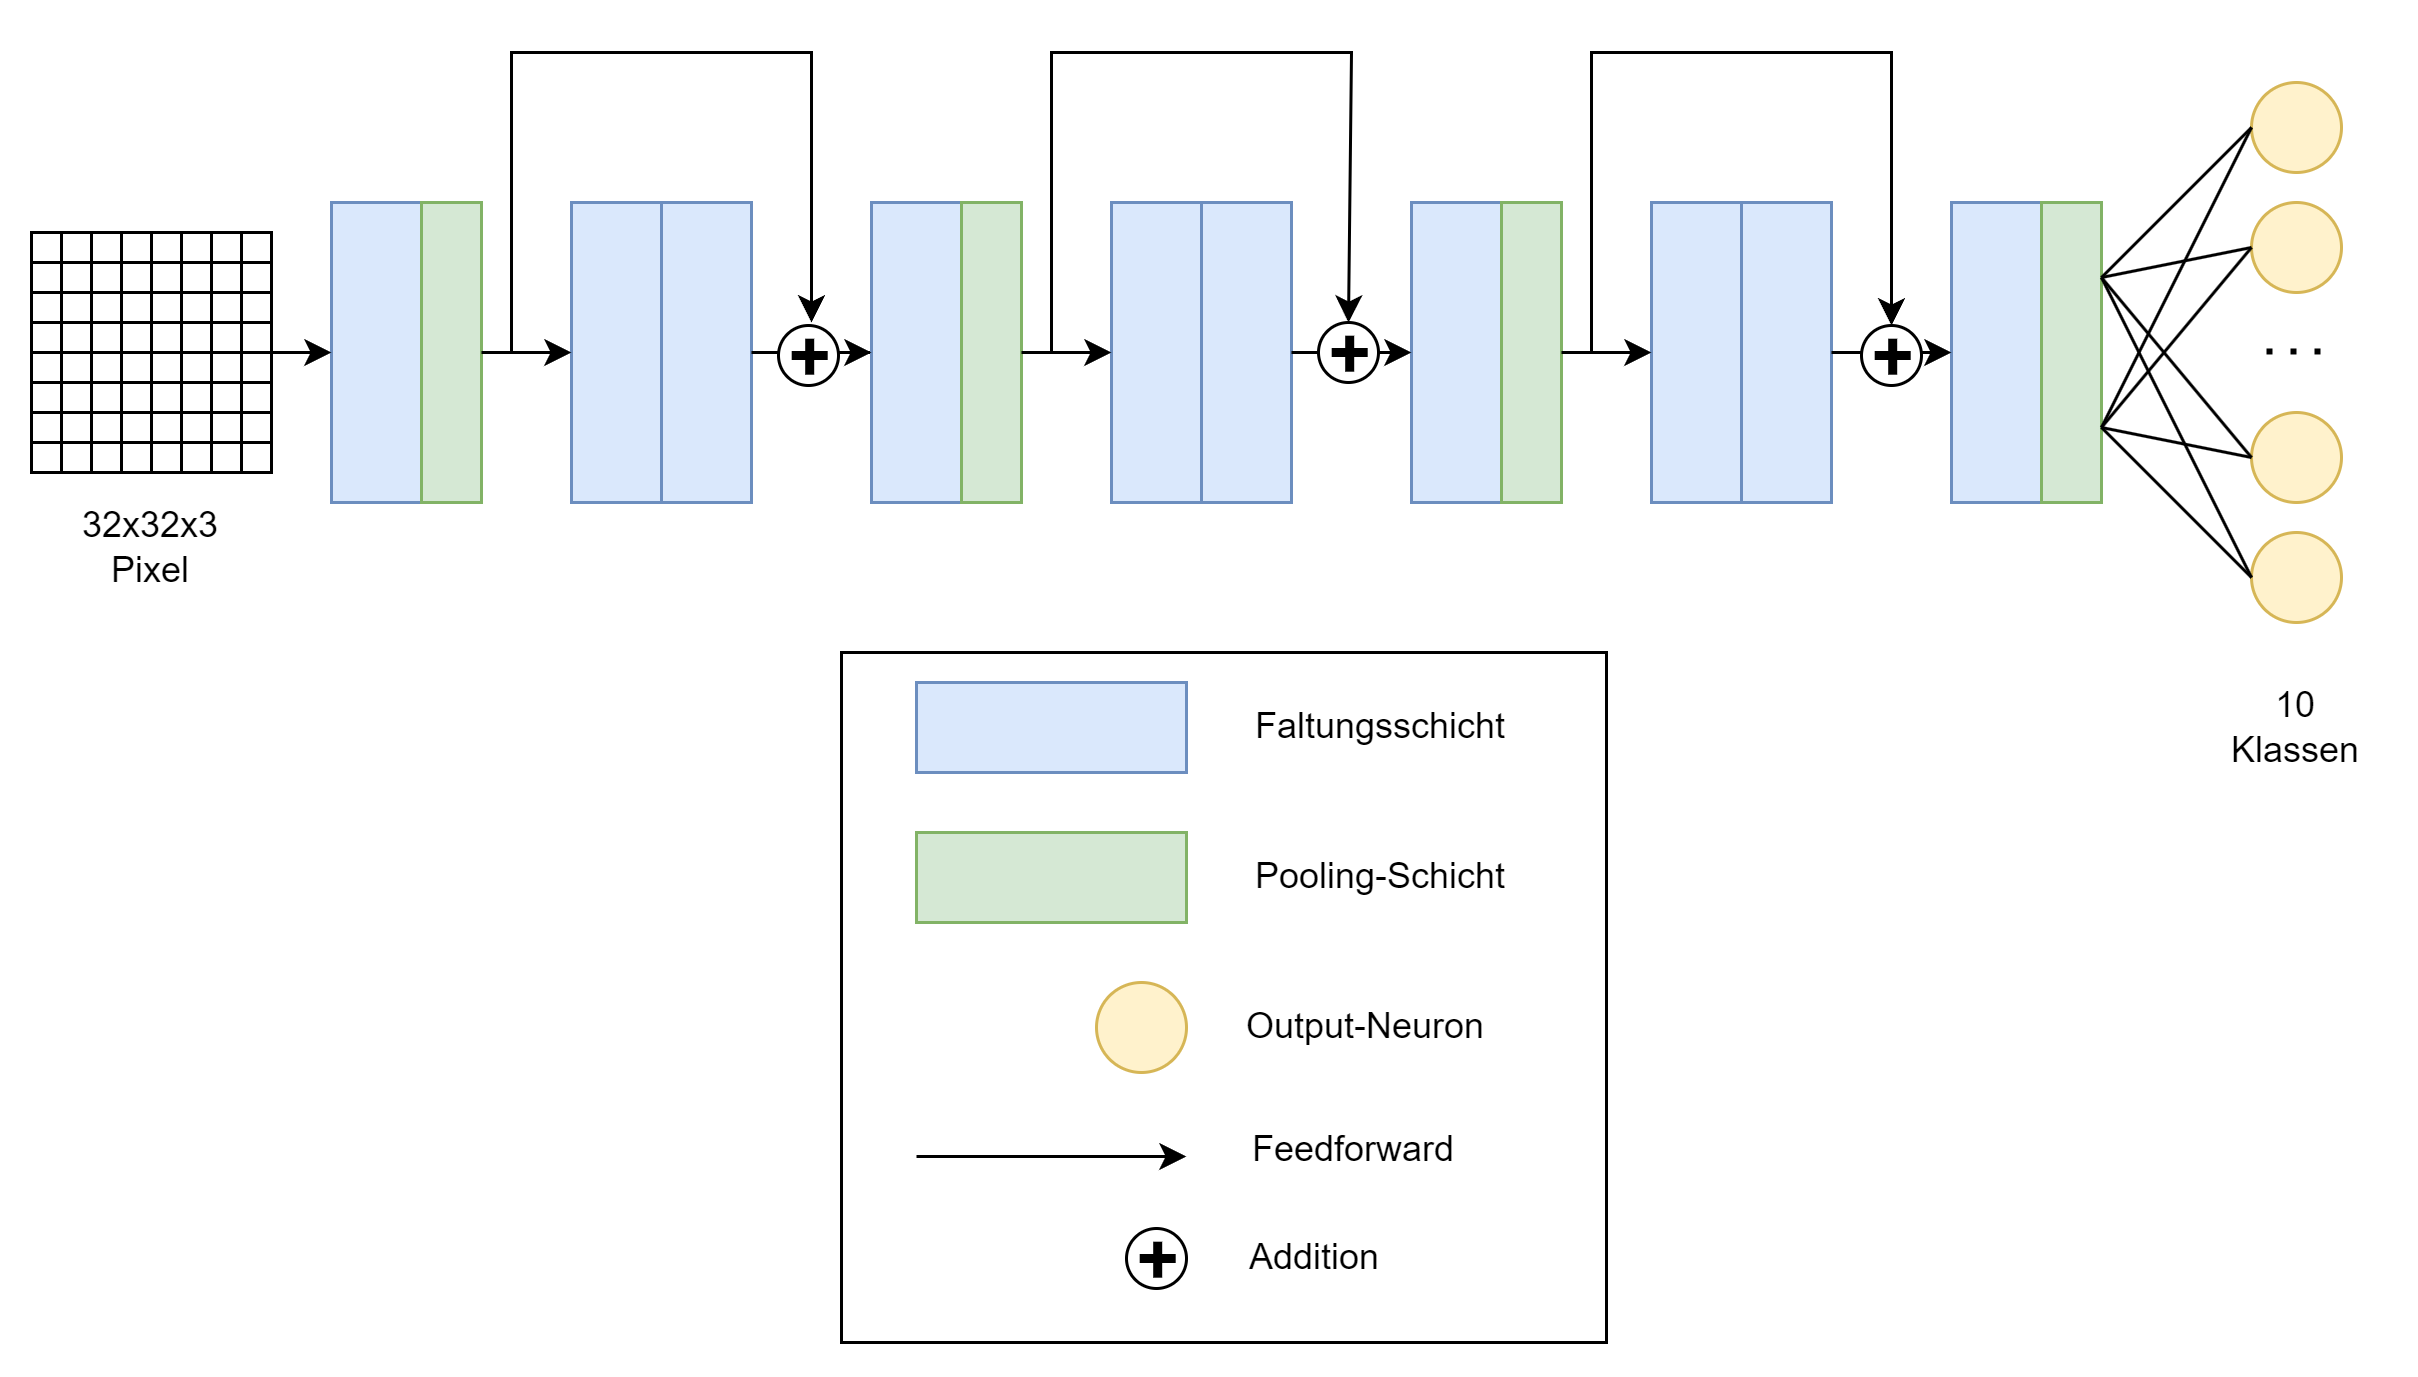
\includegraphics[width=15cm]{figures/cifar_modell.png}
    \caption{Neuronales Netz zur Klassifikation von CIFAR-10}
    \label{fig:cifar_modell}
\end{figure} 

Neben CIFAR-10, wird der CelebA Datenbestand \cite{celeba} genutzt, welcher unter anderem über die Plattform Kaggle zur Verfügung steht.
Dieser enthält 202.599 Bilder, auf welchen jeweils das Gesicht einer Person des öffentlichen Lebens zu sehen ist.
Die Bilder haben jeweils eine Auflösung von $178\times218$ Pixeln mit je 3 Farbkanälen.
Zu jedem Bild gibt es 40 Labels, wobei jedes davon eine Eigenschaft beschreibt. 
Dabei können jeweils die Werte -1 (Eigenschaft nicht vorhanden) und 1 (Eigenschaft vorhanden) angenommen werden.
Ein Beispiel für eine Eigenschaft ist die Größe eines Organs sein (Label \dq \textit{Big\_Nose}\dq).
Manche Eigenschaften können sich außerdem gegenseitig ausschließen.
So gibt es beispielsweise mehrere Labels für Haarfarben (Label \dq \textit{Black\_Hair}\dq\ und Label \dq \textit{Blond\_Hair}\dq).
Der Datenbestand ist bereits unterteilt in \dq \textit{Training}\dq, \dq \textit{Validierung}\dq\ und \dq \textit{Test}\dq.
Die vorgegebene Einteilung wird beibehalten, sodass die Güte des Modells immer auf der Testdatenmenge, welche nicht im Training genutzt werden, gemessen wird.
Tabelle \ref{tab:anzahl_datensaetze} zeigt die Anzahl der Datensätze in den jeweiligen Teildatenbeständen.

\begin{table}[!htb]
\centering
\begin{tabular}{|l|l|l|}
\hline
\rowcolor[HTML]{CBCEFB} 
{\color[HTML]{000000} Datenbestand} & Anzahl Datensätze  & prozentualer Anteil\\ \hline
Training & 162.770  &     $\approx$ 80\%  \\ \hline
Validierung & 19.867 &     $\approx$ 10\%      \\ \hline
Test  & 19.962 &    $\approx$ 10\%    \\ \hline

\end{tabular}
\caption{Anzahl Datensätze}
\label{tab:anzahl_datensaetze}
\end{table}

Der Use Case ist es dabei, alle 40 Label eines Bildes vorherzusagen.
Dabei handelt es sich um ein sogenanntes Multi-Label Klassifizierung, also eine Klassifikation bei der mehrere Klassen (hier Eigenschaften) bestimmt werden können.
Als Metrik zur Messung der Güte eines Modells wird dabei die Genauigkeit genutzt, also das Verhältnis von richtig vorhergesagten Labels zu der gesamten Anzahl an Labels.

Für diesen Use Case werden zwei unterschiedliche Modelle genutzt.
Bei dem ersten Modell handelt es sich um ein ResNet-18 Modell \cite{resnet}.
Dieses hat eine ähnliche Architektur wie das bereits beschriebene Modell für die Klassifizierung der CIFAR-10 Daten.
Jedoch besitzt dieses Modell 18 Faltungsschichten, wodurch die Anzahl der Parameter größer ist.
Das zweite Modell ist das sogenannte Vision Transformer Modell \cite{vit}, kurz ViT. 
Dieses Modell nutzt einige Elemente der Transformer-Architektur, welche ursprünglich aus dem Bereich der Computerlinguistik stammt \cite{transformer}. 
Das Vision Transformer Modell unterteilt das Bild in mehrere, gleich große Teilbilder, welche Patches genannt werden.
Dabei erhalten die Patches eine Position, welche von oben links nach unten rechts inkrementiert wird.
Die Patches werden über sogenannte Embedding-Schichten in einen höherdimensionalen Vektorraum übertragen.
Die entstandenen Vektoren werden Embeddings genannt.
Im Laufe des Trainingsprozesses, werden die Parameter der Embedding-Schichten so angepasst, dass die Ähnlichkeit zweier Embeddings mit der Ähnlichkeit der Eingabebilder korreliert. 
Die Embeddings werden anschließend mit der Position der jeweiligen Patches als Eingabe für einen oder mehrere sequentiell verbundene Kodierer, auch Encoder genannt, genutzt.
Diese bestehen aus jeweils mindestens einem Aufmerksamkeitsmechanismus, auch Attention genannt, und einigen vollständig verbundenen Schichten eines neuronalen Netzes.
Die Aufmerksamkeitsmechanismen erlernen verschiedene Beziehungen der Patches zueinander, welche durch die jeweiligen Positionen in einer räumlichen Verbindung stehen.
Die Ausgabe des letzten Kodierers wird anschließend als Eingabe für vollständig verbundene Schichten genutzt, welche die Klassifikation durchführen.
Neuronen der letzten Schicht repräsentieren jeweils eine Klasse.